\documentclass{beamer}

\setbeameroption{show notes on second screen=right}
\setbeamercolor{frame number in head/foot}{fg=black}
\setbeamerfont{frame number in head/foot}{size=\small}
\setbeamertemplate{note page}[plain]
\setbeamertemplate{navigation symbols}{}
\setbeamertemplate{footline}[frame number]

\usepackage{hyperref,xcolor,tikz,listings}
\usepackage{amsmath,amssymb,amsfonts,amsthm}
\usepackage{multirow,longtable,booktabs,array}
% fonts
\usepackage{fontspec}
\usepackage[T1]{fontenc}
\usepackage[tt=false, type1=true]{libertine}
\usepackage[libertine]{newtxmath}
% misc
\usepackage{xfrac}
\usepackage{graphicx}
\usepackage{float,caption,subcaption} % support \subfigure and \begin{figure}[H] https://tex.stackexchange.com/a/299246 


\usepackage{import}
\usepackage{changepage}
\usepackage{mathtools} % \xmapsto

\definecolor{red}{HTML}{C63A44}
\usetikzlibrary{decorations.pathreplacing}
\captionsetup{justification=raggedright,singlelinecheck=false}
\hypersetup{colorlinks=true,linkcolor=blue,urlcolor=cyan}

\newcommand\sube\subseteq
\newcommand\supe\supseteq
\renewcommand\sup\supset
\newcommand\gt>
\newcommand\lt<
\renewcommand\ge\geqslant 
\renewcommand\geq\geqslant 
\renewcommand\le\leqslant 
\renewcommand\leq\leqslant 
\newcommand\rarr\rightarrow

\setmonofont{iosevka-custom-regular.ttf}
\setlength\parindent{0pt}

\graphicspath{{figures/}}
\newcommand\g[2][0.2]{\raisebox{-0.45\height}{\includegraphics[width=#1\columnwidth]{#2}}}

\title{A Computational Approach to String Figures}
\date{2023-11-29}
\author{Yulong Liu}
\begin{document}
\maketitle


\section{String Figures}

\begin{frame}{\secname}
\begin{itemize}
    \item Designs formed from a loop of string
    \item Commonly known as a children's game
\end{itemize}

\pause People have been playing with the string around the world for millennia.

\begin{itemize}[<+(1)->]
    \item  Entertainment during polar nights in the Arctic region
    \item  Storytelling and illustrating scenes from myths and legends
\end{itemize}

\textcolor{red}{todo insert 3 images of strings figures from the encyclopedia: the star, something i can do, something i cant do}
\end{frame}

\note[itemize]{
\item the native inhabitants in the arctic region play string figures for entertainment durong polar nights
\item the indigenous people in New Zealand play string figures for storytelling and illustrating scenes from myths and legends
\item and i play string figures when overleaf takes forever to compile my slides
}


\begin{frame}{A Computational Approach}
String figures take a lot of steps to make

\begin{itemize}[<+(1)->]
    \item  Start with an initial position
    \item  Apply a sequence of moves
    \item  Each move transforms a string figure to another
\end{itemize}

\pause String figures computations

\begin{itemize}[<+(1)->]
    \item  Represent string figures: simple, precise
    \item  Apply moves directly to the representations
\end{itemize}

\pause Motivation

\begin{itemize}[<+(1)->]
    \item Do string figures on paper
    \item Computer simulations \& animations
\end{itemize}

\end{frame}

\note[itemize]{
\item (take steps) for example, to make the star, we start with this initial position, and then apply two simple moves of picking a segment of the string 
\item (mot) clear way of describing how to make string figures
\item (mot) teach computers how to play string figures
\item (record) store in computer, as database
\item simliar to music scores, rubiks cubes
\item one effective way of describing string figures is to draw them, as string diagrams
}
\newcommand\w[1]{\includegraphics[width=0.3\textwidth]{#1}}

\section{Representation}

\subsection{Diagrams}
\begin{frame}{\secname: \subsecname}
Fingers are named $L1,\cdots, L5$ and $R1,\cdots,R5$ from thumb to pinky

\begin{itemize}
    \item \pause Ordered from nearest to furthest
    \pause \begin{center}
    $L1\lt L2\lt L3\lt L4\lt L5$\\
    $R1\lt R2\lt R3\lt R4\lt R5$    
    \end{center}
\end{itemize}

\pause String segments are named by finger $F\in\{L1,\cdots, L5,R1,\cdots,R5\}$
\begin{itemize}[<+(1)->]
    \item $Fn$ is the near string, $Ff$ is the far string
    \item $Lp$ and $Rp$ are palmar strings
\end{itemize}

\pause
\begin{figure}\centering
\def\svgwidth{0.5\columnwidth}
\input{figures/open.pdf_tex}
\end{figure}

\note[item]{ (eg) top down view}
\note[item]{ (palmar) when we have a string between $L1$ and $L5$, we give a special name, called palmar string}
\note[item]{ the diagrams are intuitive and very visual, but they are less computer friendly}
\note[item]{ what do computers like? they like array of symbols}

\end{frame}


\subsection{Linear Sequences}
\begin{frame}{\secname: \subsecname}
Two key components
\begin{itemize}[<+(1)->]
    \item Fingers that hold the string
    \item Crossings (with parity)
\end{itemize}

\pause Diagram $\to$ linear sequence

\begin{itemize}[<+(1)->]
    \item Start with left nearest finger and travel clockwise
    \item Visit fingers and crossings (with parity)
\end{itemize}

\def\svgwidth{0.6\columnwidth}
$$\begin{tikzpicture}
    \node at(0,0){\input{figures/open.pdf_tex}};
    \node[shift={(120pt,0)}] at(0,0){$\mapsto$};
    \node[shift={(170pt,0)}] at(0,0){$L1:L5:R2$};
\end{tikzpicture}$$
\note[item]{travel along the string clockwise}
\note[item]{note down the fingers and crossings with parity}
\end{frame}


\begin{frame}{Linear Sequences with Crossings}
Diagram $\to$ linear sequence
\begin{itemize}[<+(1)->]
    \item Name each crossing as $x_i$ for some $i$
    \item Visit overcrossing $\implies$ write $x_i(o)$
    \item Visit undercrossing $\implies$ write $x_i(u)$
\end{itemize}

\pause
$$\begin{tikzpicture}
    % \node at(0,0){\def\svgwidth{0.6\columnwidth}\input{figures/star.pdf_tex}};
    \node at(0,0){\def\svgwidth{0.6\columnwidth}\input{figures/starc.pdf_tex}};
\end{tikzpicture}$$

$$
\scriptstyle
L1:x_1(o):x_2(o):R5:x_3(o):x_4(o):R1:x_5(o):x_1(u):L5:x_2(u):x_3(u):R2:x_4(u):x_5(u)
$$

\note[item]{if we have $n$ fingers holding the string figure that has $m$ crossings, the sequence will have $n+2m$ symbols}
\note[item]{in most string figures, having a lot of crossings is what makes them beautiful, and it would be tedious to write down the entire sequence by hand}
\note[item]{(you see that i cant even fit the linear sequence of this simple star with normal size font)}
\note[item]{so this gives us more motivation to develop a systematic way of computing the movements so we can let computer do the calculuation}
\note[item]{the most common movements involve a finger and sometimes a near/far string segment of some other finger, but the problem arises in identifying these segments from the sequence}

\end{frame}



\subsection{Identifying String Segments }

\begin{frame}{\subsecname from Linear Sequences}
\begin{adjustwidth}{-1.5em}{-1.5em}
Consider a subsequence $\ldots:L_i:\ldots$ for any $L_i\in\{L1,\ldots,L5\}$

\begin{itemize}[<+(1)->]
    \item Traverse clockwise \raisebox{-0.45\height}{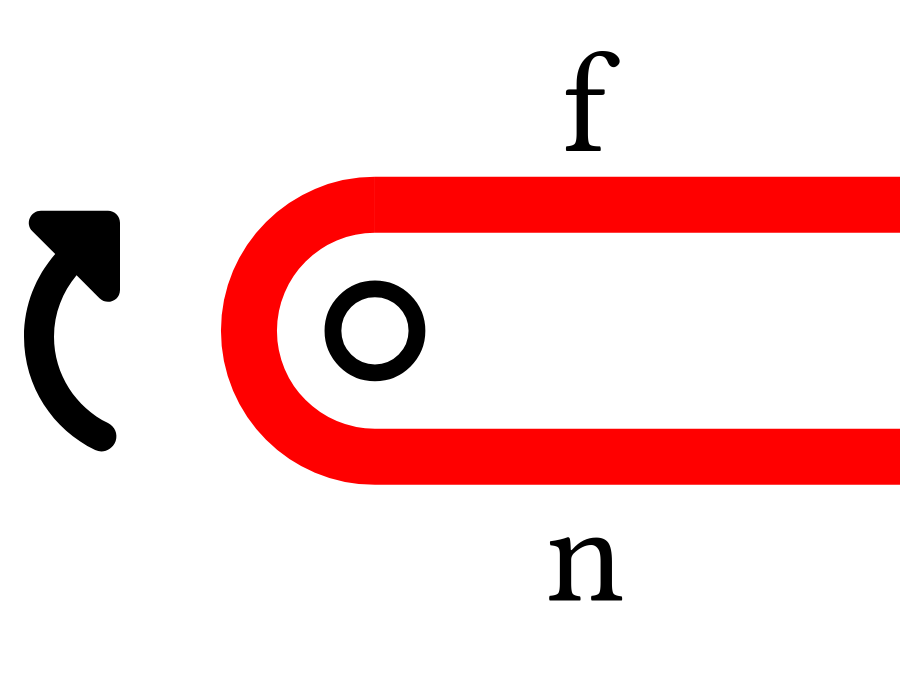
\includegraphics[width=0.2\textwidth]{figures/leftcw.png}} \pause $\implies \ldots:[L_in] L_i [L_if]:\ldots$
    \item Traverse counterclockwise \raisebox{-0.45\height}{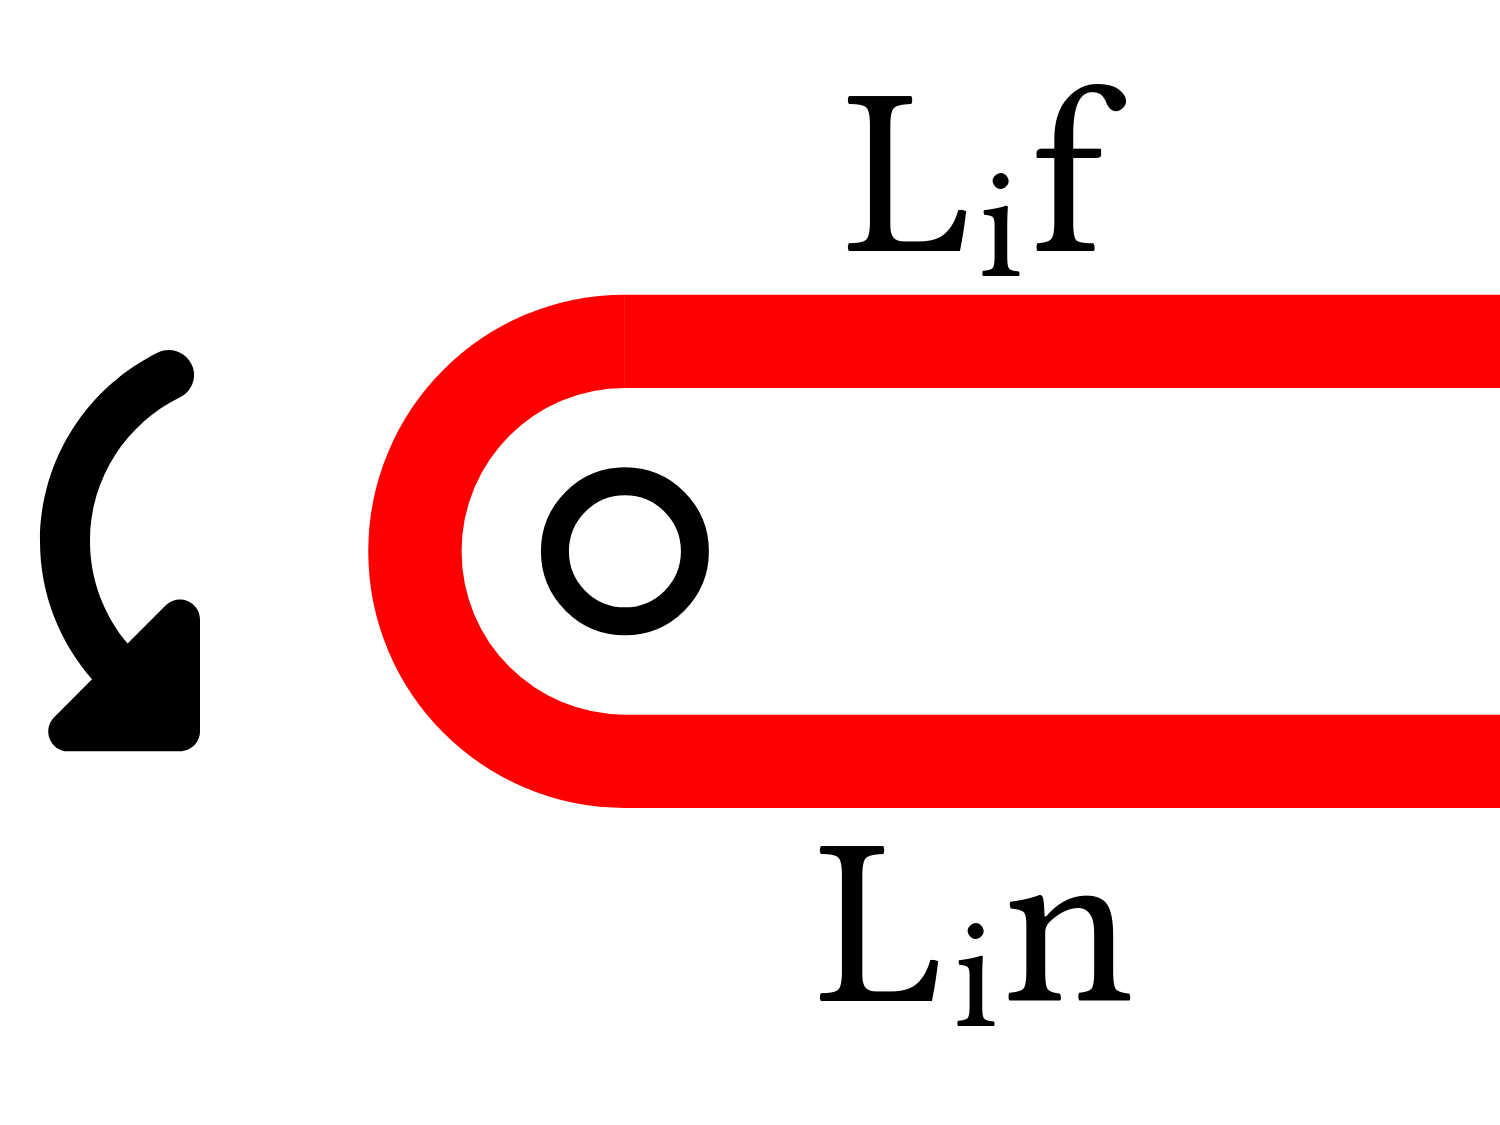
\includegraphics[width=0.2\textwidth]{figures/leftccw.png}} \pause $\implies\ldots: [L_if] L_i [L_in]:\ldots$
\end{itemize}

\pause Similarly for finger $R_i$ on the right hand

\begin{itemize}
    \item \raisebox{-0.45\height}{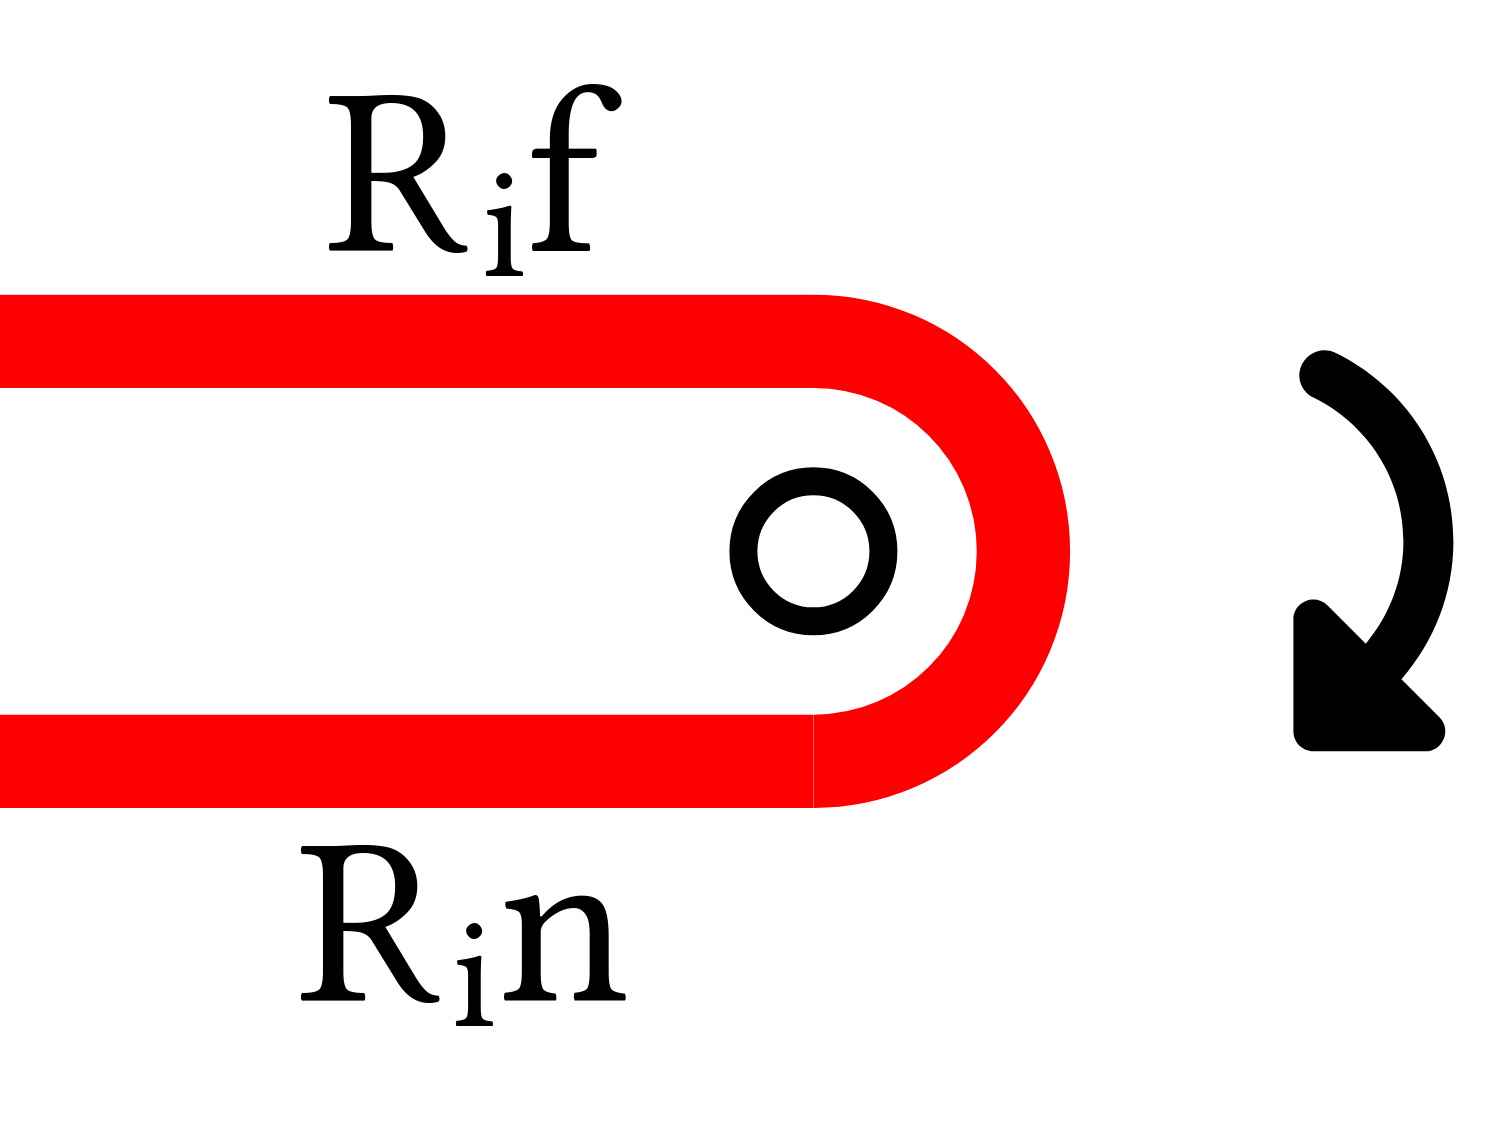
\includegraphics[width=0.2\textwidth]{figures/rightcw.png}} $\implies \ldots:[R_if]R_i[R_in]:\ldots$
    \item\raisebox{-0.45\height}{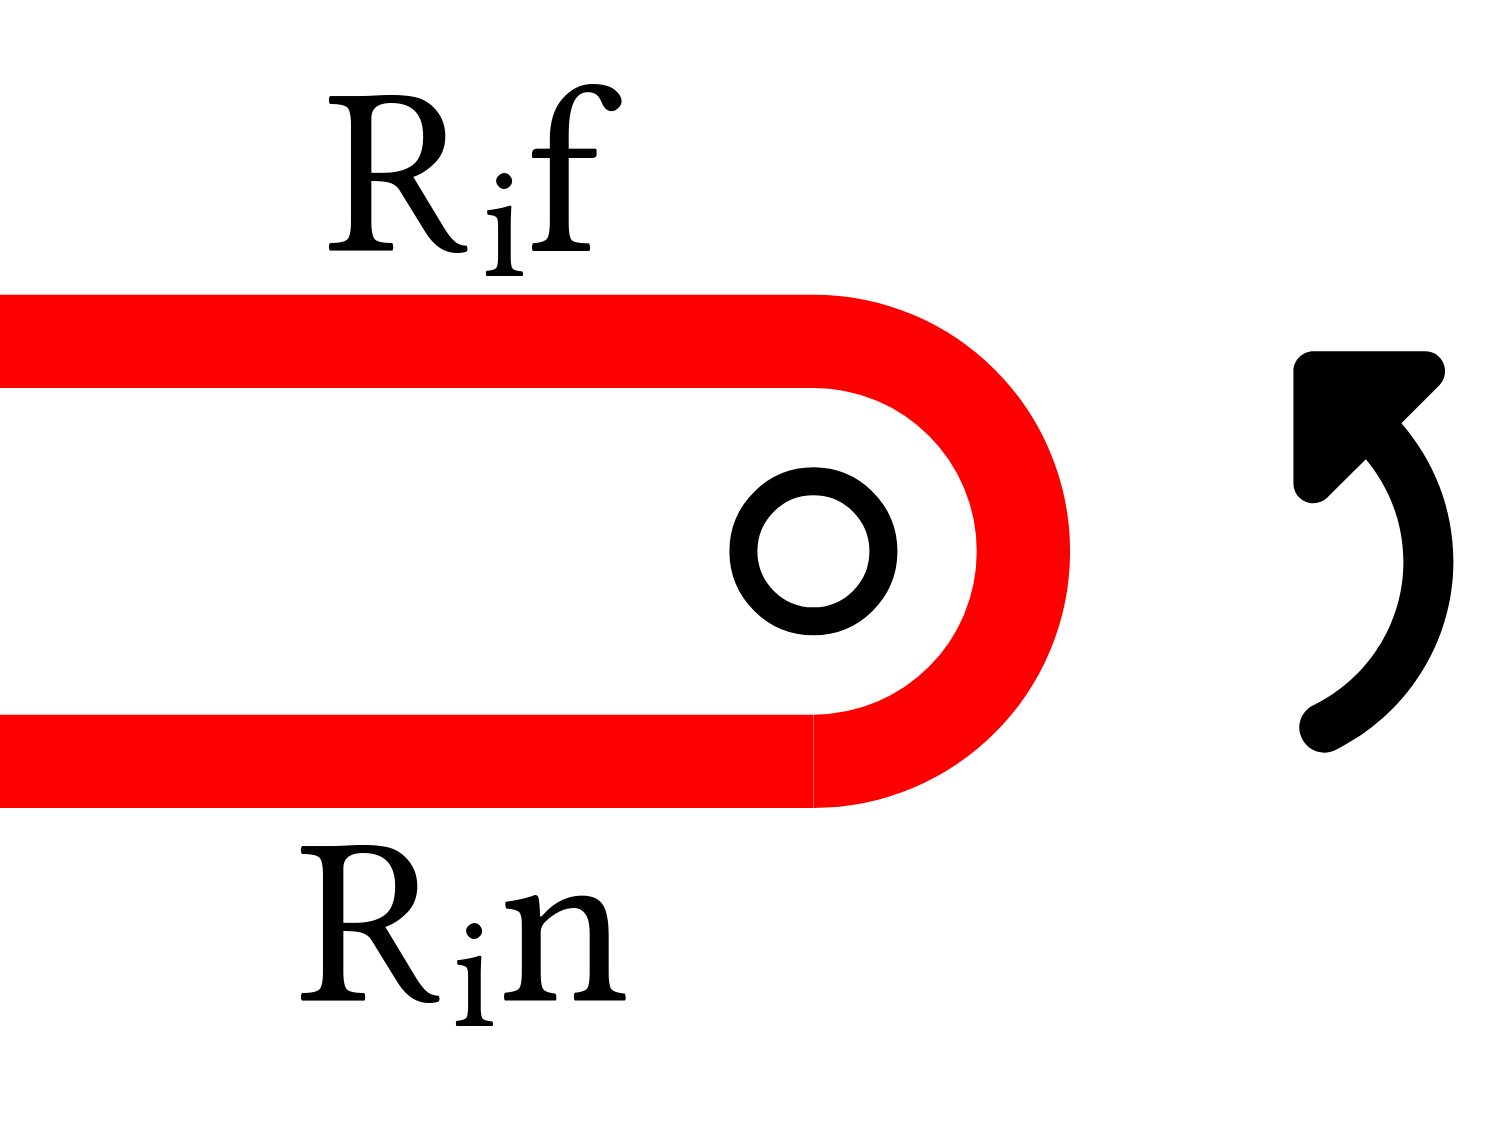
\includegraphics[width=0.2\textwidth]{figures/rightccw.png}} $\implies\ldots:[R_in]R_i[R_if]:\ldots$
\end{itemize}
\end{adjustwidth}
\end{frame}

\begin{frame}{\subsecname: Opposite Hand}
\begin{adjustwidth}{-1.5em}{-1.5em}
Consider $\ldots:L2:\ldots:R2:\ldots$

\begin{itemize}[<+(1)->]
    \item Even number of crossings between $L2$ and $R2\implies$ rotation persists\\
    \begin{center}
    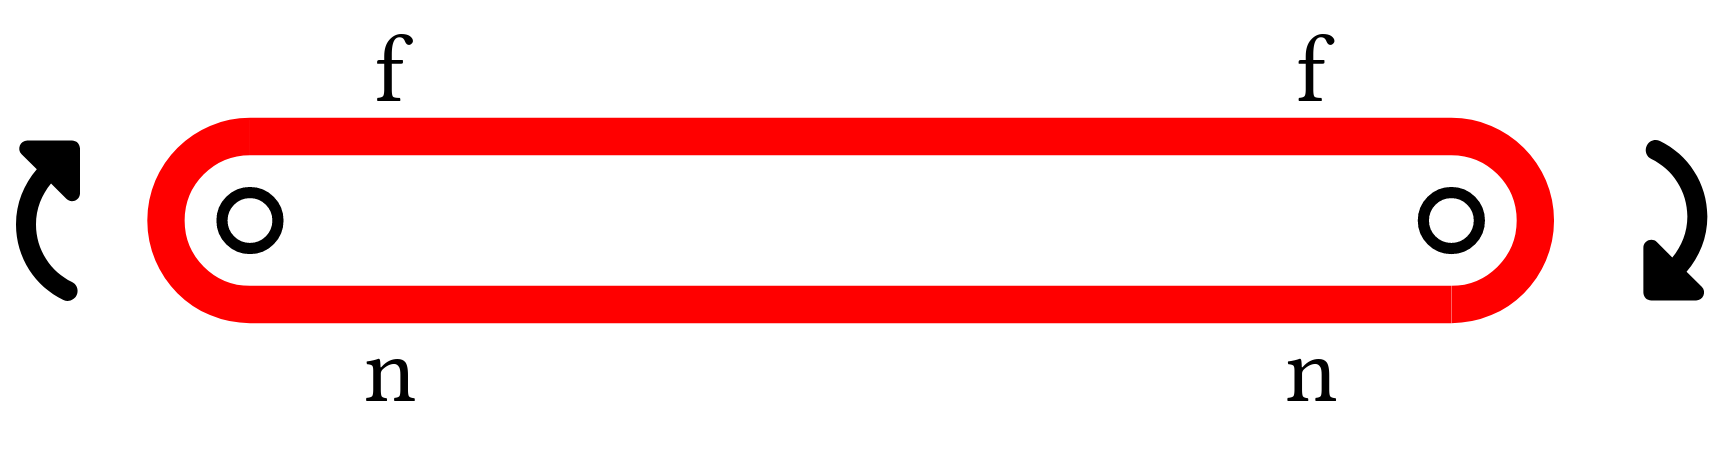
\includegraphics[width=0.5\columnwidth]{figures/diff-even.png}
    $$
    [L2n]L2[L2f]:[R2f]R2[R2n]
    $$
    \end{center}
    \item Odd number of crossings between $L2$ and $R2\implies$ rotation reverses\\
    \begin{center}
    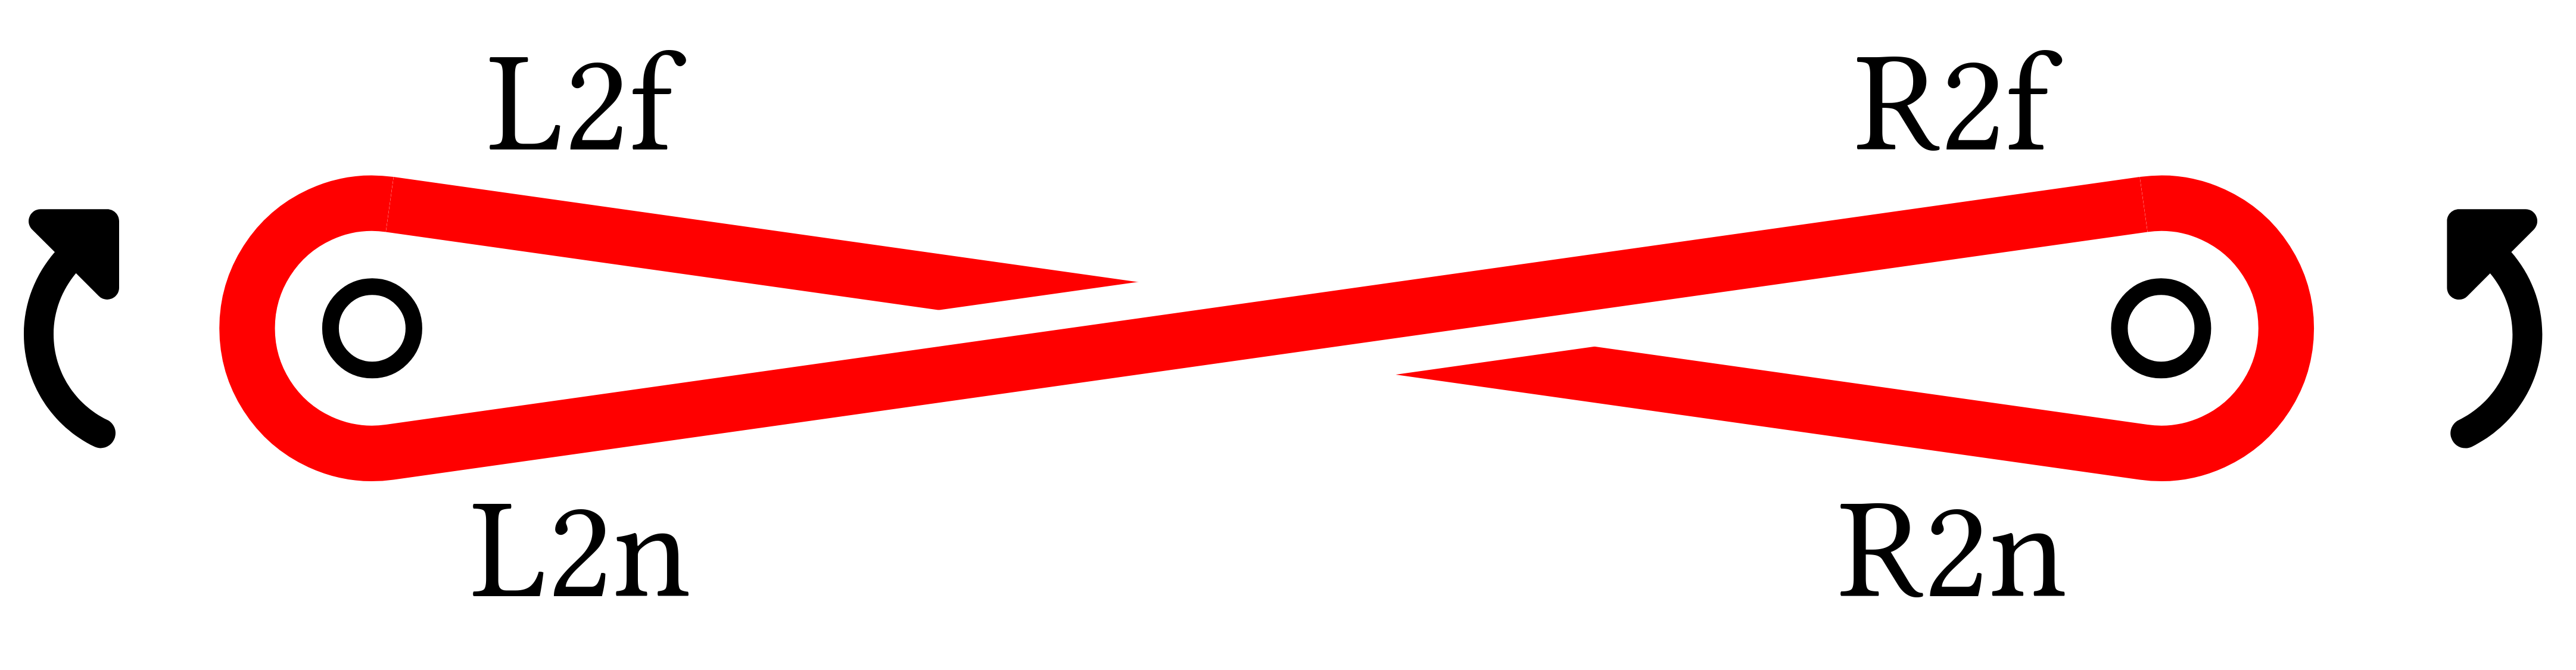
\includegraphics[width=0.5\columnwidth]{figures/diff-odd.png}
    $$
    [L2n]L2[L2f]:x_1(u):[R2n]R2[R2f]:x_1(o)
    $$
    \end{center}
\end{itemize}    
\end{adjustwidth}
\end{frame}

\begin{frame}{\subsecname: Same Hand}
\begin{adjustwidth}{-1.5em}{-1.5em}
Consider $\ldots:L2:\ldots:L5:\ldots$

\vfill
\pause
\begin{minipage}{0.5\textwidth}
\begin{center}
Even $\implies$ rotation persists\\
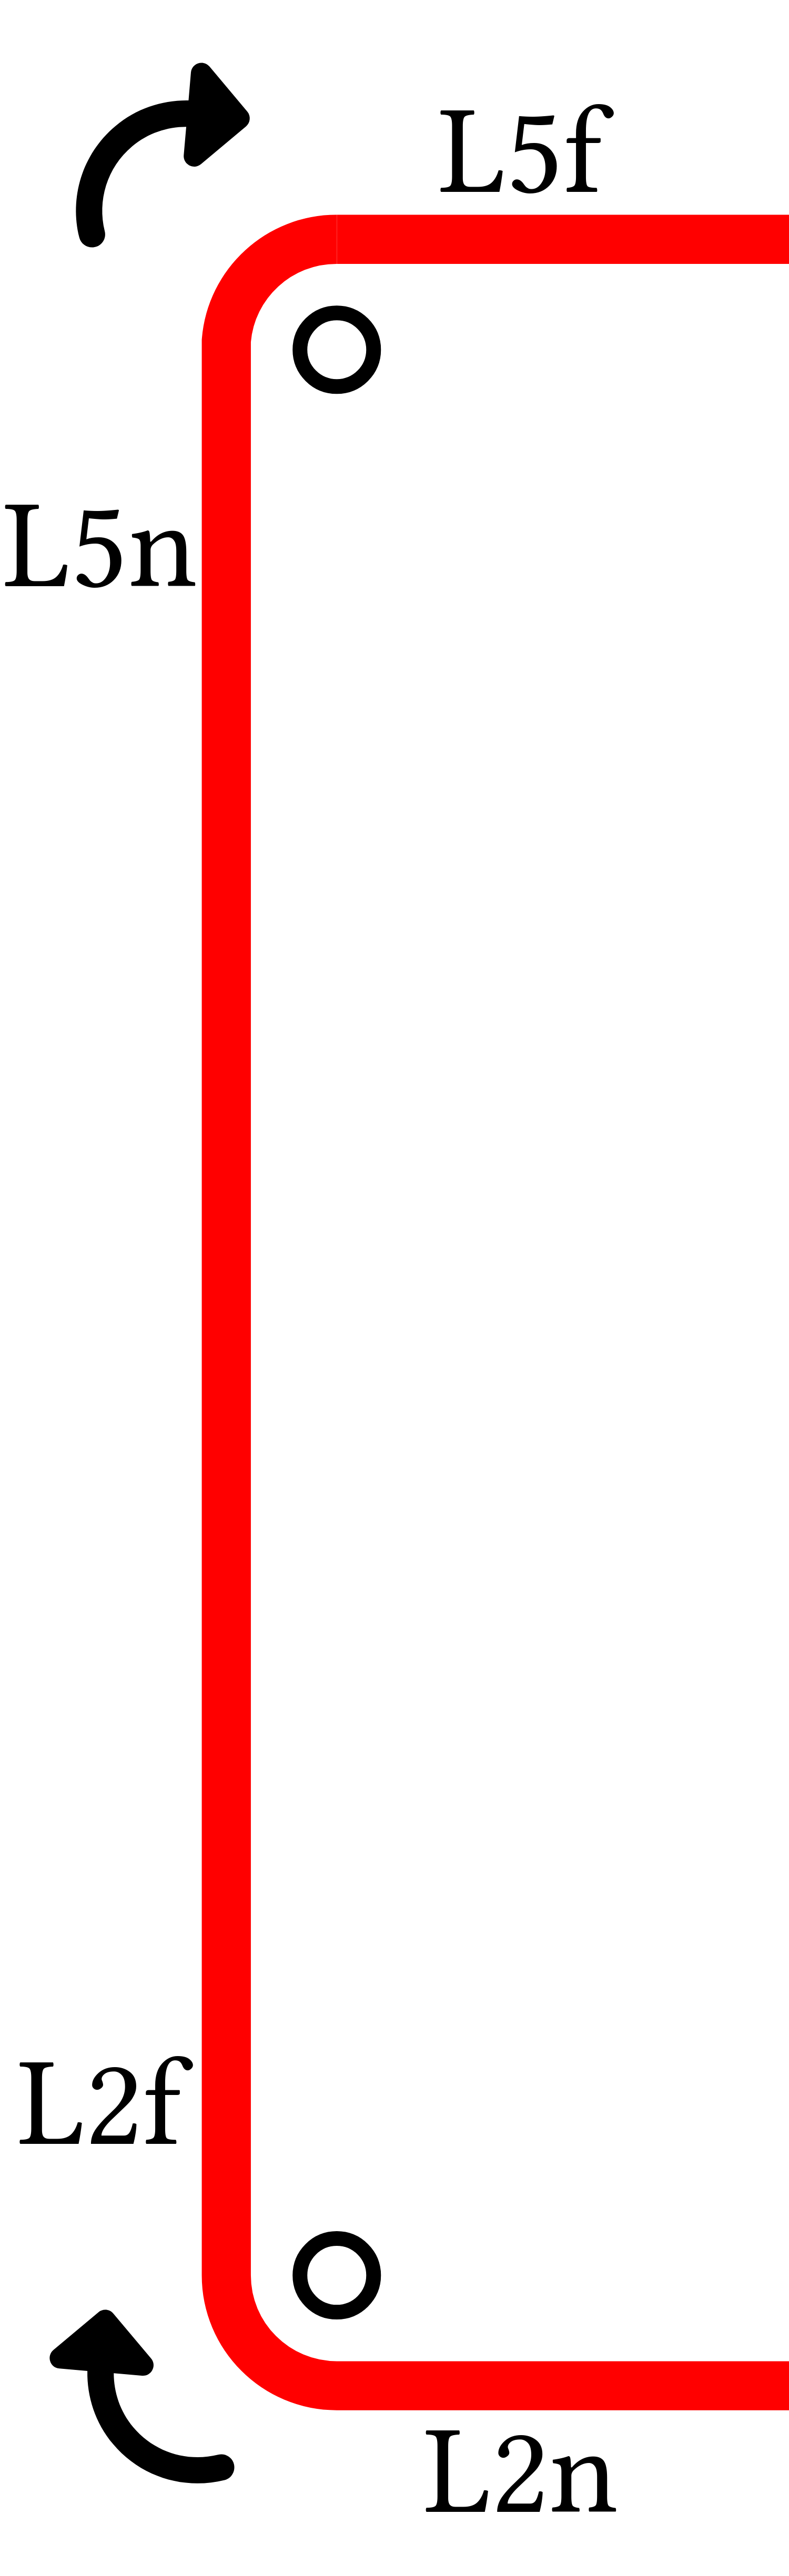
\includegraphics[width=0.3\linewidth]{figures/same-even.png}
\end{center}
$$
\scriptstyle
\ldots:[L2n]L2[L2f]:[L2n]L2[L2f]:\ldots
$$
\end{minipage}
\hfill
\pause
\begin{minipage}{0.5\textwidth}
\begin{center}
Odd $\implies$ rotation reverses\\
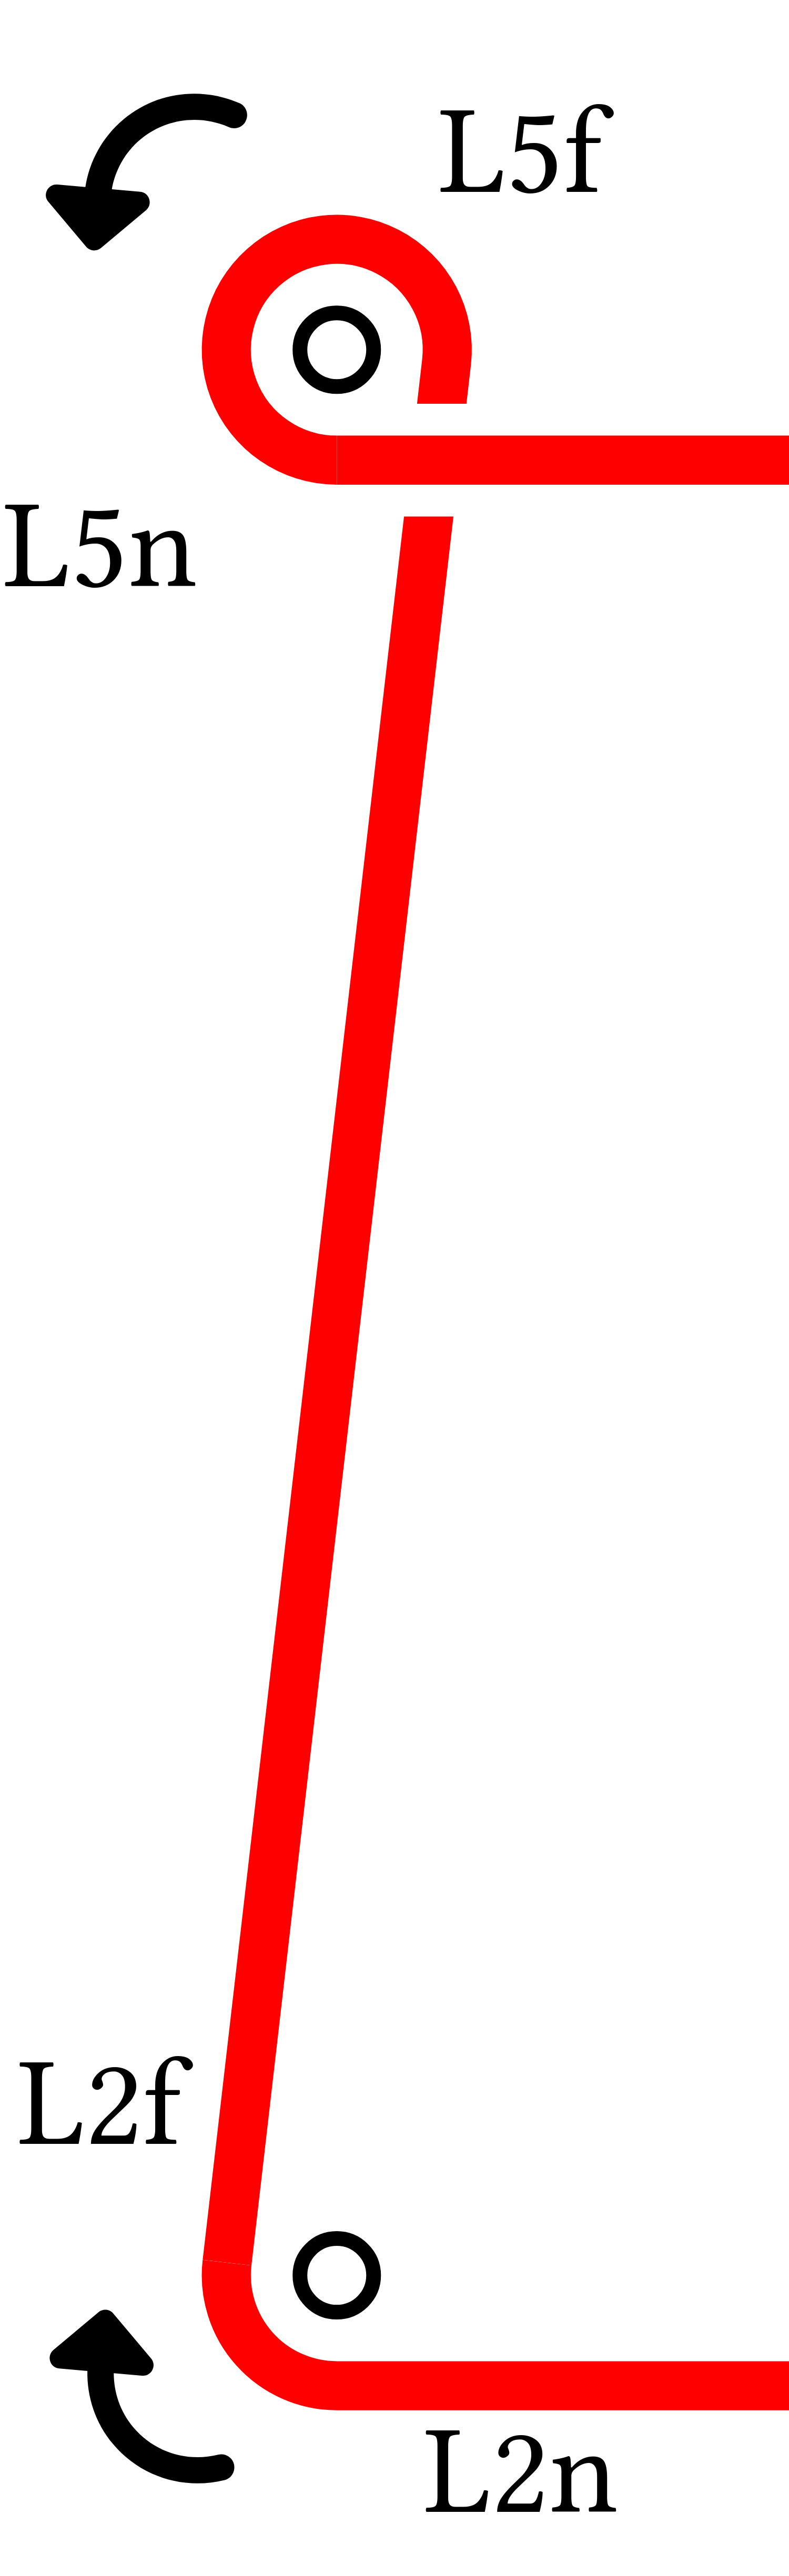
\includegraphics[width=0.3\linewidth]{figures/same-odd.png}
\end{center}
$$
\scriptstyle
\ldots:[L2n]L2[L2f]:x_1(u):[L5f]L5[L5n]:x_1(o):\ldots
$$
\end{minipage}
\end{adjustwidth}
\end{frame}

\begin{frame}[t]{\subsecname: Example}

$$
{L1}:x_1(o):R5:x_2(o):L5:x_2(u):x_1(u):R2
$$

\pause {By convention, the first finger in the linear sequence is clockwise}

\begin{adjustwidth}{-2em}{-2em}
$$
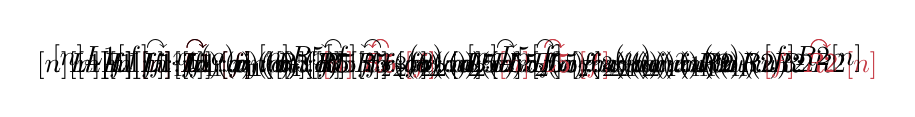
\begin{tikzpicture}
    \node at(0,0){$\stackrel{\phantom\curvearrowright}{L1}:x_1(o):R5:x_2(o):L5:x_2(u):x_1(u):R2$};
    \node<+> at(0,0){${\color{red}\stackrel\curvearrowright{L1}}:x_1(o):R5:x_2(o):L5:x_2(u):x_1(u):R2$};
    \node<+> at(0,0){${\color{red}[n]\stackrel\curvearrowright{L1}[f]}:x_1(o):R5:x_2(o):L5:x_2(u):x_1(u):R2$};
    \node<+> at(0,0){$[n]\stackrel\curvearrowright{L1}[f]:x_1(o):{\color{red}\stackrel\curvearrowleft{R5}}:x_2(o):L5:x_2(u):x_1(u):R2$};
    \node<+> at(0,0){$[n]\stackrel\curvearrowright{L1}[f]:x_1(o):{\color{red}[n]\stackrel\curvearrowleft{R5}[f]}:x_2(o):L5:x_2(u):x_1(u):R2$};
    \node<+> at(0,0){$[n]L1[f]:x_1(o):[n]\stackrel\curvearrowleft{R5}[f]:x_2(o):{\color{red}\stackrel\curvearrowright{L5}}:x_2(u):x_1(u):R2$};
    \node<+> at(0,0){$[n]L1[f]:x_1(o):[n]\stackrel\curvearrowleft{R5}[f]:x_2(o):{\color{red}[n]\stackrel\curvearrowright{L5}[f]}:x_2(u):x_1(u):R2$};
    \node<+> at(0,0){$[n]L1[f]:x_1(o):[n]R5[f]:x_2(o):[n]\stackrel\curvearrowright{L5}[f]:x_2(u):x_1(u):{\color{red}\stackrel\curvearrowright{R2}}$};
    \node<+> at(0,0){$[n]L1[f]:x_1(o):[n]R5[f]:x_2(o):[n]\stackrel\curvearrowright{L5}[f]:x_2(u):x_1(u):{\color{red}[f]\stackrel\curvearrowright{R2}[n]}$};
    \node<+-> at(0,0){$[n]L1[f]:x_1(o):[n]R5[f]:x_2(o):[n]{L5}[f]:x_2(u):x_1(u):[f]{R2}[n]$};
\end{tikzpicture}
$$
\end{adjustwidth}

\only<4->{
\begin{center}
\begin{tabular}{c|c}
    \w{figures/leftcw.png}&\w{figures/rightcw.png}\\
    \hline
    \w{figures/leftccw.png}&\w{figures/rightccw.png}\\
\end{tabular}
\end{center}
}
\only<12>{todo erase table, show string figure}

\note[item]{now that we can recover the string segments from the linear sequence}
\note[item]{when we want to pick a specific string segment, we know where it is in the linear sequence}
\note[item]{"use a finger to pick some segment" is essentially insert the finger to where the segment is in the linear sequence along with some crossings if needed}

\end{frame}


\section{Moves}
\subsection{Twist}
\newcommand\g[2][0.2]{\raisebox{-0.45\height}{\includegraphics[width=#1\columnwidth]{#2}}}

\begin{frame}{\secname: \subsecname}
\pause Two variations: twist towards and twist away
\begin{itemize}[<+(1)->]
    \item Twist the loop on finger $F$ \emph{towards} player: $<F$
    \item Twist the loop on finger $F$ \emph{away} from player: $>F$
\end{itemize}
\pause Consider $\ldots:[Fn]F[Ff]:\ldots$
\begin{itemize}[<+(1)->]
    \item\g[0.15]{figures/twist-before} $\quad\stackrel{<F}\mapsto\quad$ \g[0.15]{figures/twist-towards}
    $$
    \ldots:[Fn]F[Ff]:\ldots\quad\stackrel{<F}\mapsto\quad\ldots:x(u):F:x(o):\ldots
    $$
    \item \g[0.15]{figures/twist-before} $\quad\stackrel{<F}\mapsto\quad$ \g[0.15]{figures/twist-away}
    $$
    \ldots:[Fn]F[Ff]:\ldots\quad\stackrel{>F}\mapsto\quad\ldots:x(o):F:x(u):\ldots
    $$
\end{itemize}
\pause $\ldots:[Ff]F[Fn]:\ldots\implies$ crossing parities are reversed
\end{frame}

\note[itemize]{
\item Storer p382
\item works on right hand too
}

\subsection{Pick}
\begin{frame}{\secname: \subsecname}

Finger $F$ picks a string segment $s$ 

\begin{itemize}
    \item Written as $F(s)$
\end{itemize}

\pause Two types of variations:
\begin{itemize}[<+(1)->]
    \item $F$ passes \emph{over/under} all intermediate segments
    \item $F$ picks $s$ from \emph{above/below}
\end{itemize}

\pause Examples
\begin{itemize}[<+(1)->]
    \item "$R5$ passes \emph{over} all intermediate segments and picks $Lp$ from \emph{above}" is denoted  as $\overset\Longleftarrow{R5}(\overline{Lp})$
    \item "$R1$ passes \emph{over} all intermediate segments and picks $R5n$ from \emph{below}" is denoted as $\overrightarrow{R1}(\underline{R5n})$
    \item "$R4$ passes \emph{below} all intermediate segments and picks $L1n$ from \emph{below}" is denoted as $\overset\Longleftarrow{R4}(\underline{L1n})$
\end{itemize}
\end{frame}

\note[itemize]{
\item the first 2 moves makes the star
\item pick moves can be really hard to perform in reality, e.g. apply 3rd one after 1 and 2
}

\begin{frame}{\subsecname: Examples}
\begin{adjustwidth}{-2em}{-2em}
\begin{minipage}{0.7\columnwidth}
\pause \g{figures/pick-before}$\enspace\xmapsto{\underleftarrow{R5}(\underline{R1n})}\enspace$ \g{figures/pick-under-below}\\
\pause \g{figures/pick-before}$\enspace\xmapsto{\underleftarrow{R5}(\overline{R1n})}\enspace$ \g{figures/pick-under-above}\\
\pause \g{figures/pick-before}$\enspace\xmapsto{\overleftarrow{R5}(\underline{R1n})}\enspace$ \g{figures/pick-over-below}\\
\pause \g{figures/pick-before}$\enspace\xmapsto{\overleftarrow{R5}(\overline{R1n})}\enspace$ \g{figures/pick-over-above}\\
\end{minipage}
\begin{minipage}{0.4\columnwidth}
\pause Observations
\begin{itemize}[<+(1)->]
    \item A pair of crossings for each intermediate string
    \item $F(\overline s)$ and $F(\underline s)$ differ by a twist
    \item $\overleftarrow F(s)$ and $\underleftarrow F(s)$ differ by crossing parity
\end{itemize}
\end{minipage}
\end{adjustwidth}
\end{frame}

\note[itemize]{
\item when $F$ moves towards, the new twist is a twist towards
\item when $F$ moves away, the new twist is away, e.g. $L5:R5$ and pick with $R1$
}

\begin{frame}{\subsecname: Construction}
General steps for $F(s)$
\begin{itemize}[<+(1)->]
    \item Identify intermediate segments ($Fn<F<Ff$)
    \item Insert a pair of crossings for each intermediate segment
    \item Insert $F$ at $s$ with crossings (aka Spike)
    \item Add twist if pick from above
\end{itemize}

\g[0.27]{figures/star-before}
\uncover<3->{$\mapsto$\g[0.27]{figures/star-pick}}
\uncover<5->{$\mapsto$\g[0.27]{figures/star-pick-twist}}
\end{frame}
\note[itemize]{
\item note that we can check if a move is valid since we know how to identify all the segments in a seq
}

\newcommand\name{\subsecname: Construction Example}
\begin{frame}{\name}
$L1:L5:R2\enspace\xmapsto{\overset\Longleftarrow{R5}(\overline{Lp})}\enspace???$

\begin{itemize}[<+(1)->]
    \item\raisebox{-0.30\height}{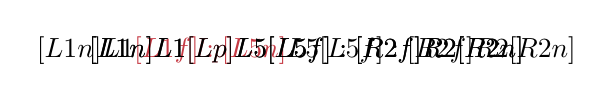
\begin{tikzpicture}
        \node<1> at(0,0){$[L1n]L1{\color{red}[L1f]:[L5n]}L5[L5f]:[R2f]R2[R2n]$};
        \node<2> at(0,0){$[L1n]L1{\color{red}[Lp]}L5[L5f]:[R2f]R2[R2n]$};
        \node<3> at(0,0){$[L1n]L1[Lp]L5[L5f]:[R2f]R2[R2n]$};
    \end{tikzpicture}}
    \item Only the segment $[L5f]:[R2f]$ is intermediate\\
    $${\color{red}Lp}=L5n<L5f=R2f<R2<{\color{red}R5}$$
\end{itemize}
\begin{center}
\g[0.6]{figures/star-before}
\end{center}
\end{frame}

\begin{frame}{\name}
$L1:L5:R2\enspace\xmapsto{\overset\Longleftarrow{R5}(\overline{Lp})}\enspace???$\\
\vfill
\pause Found $[L5f]:[R2f]$ as an intermediate segment
\begin{itemize}
    \item\pause Insert crossings $x_1$ and $x_2$
    $$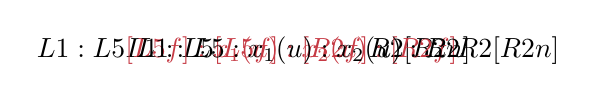
\begin{tikzpicture}
        \node<+> at(0,0){$L1:L5{\color{red}[L5f]:[R2f]}R2[R2n]$};
        \node<+> at(0,0){$L1:L5{\color{red}[L5f]:x_1(u):x_2(u):[R2f]}R2[R2n]$};
        \node<+-> at(0,0){$L1:L5:x_1(u):x_2(u):R2$};
    \end{tikzpicture}$$
\end{itemize}

\pause {Make spike for $R5$ and insert at $Lp$}

\begin{itemize}
    \item Spike: $x_2(o):R5:x_1(o)$
    $$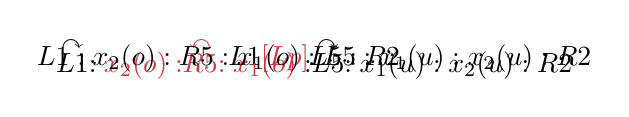
\begin{tikzpicture}
        \node<+> at(0,0){$L1{\color{red}[Lp]}L5:R2$};
        \node<+> at(0,0){$\stackrel\curvearrowright{L1}:{\color{red}x_2(o):\stackrel\curvearrowleft{R5}:x_1(o)}:\stackrel\curvearrowright{L5}:x_1(u):x_2(u):R2$};
        \node<+-> at(0,0){$L1:x_2(o):R5:x_1(o):L5:x_1(u):x_2(u):R2$};
    \end{tikzpicture}$$
\end{itemize}

\pause {Make twist on $R5$ (towards)}
$$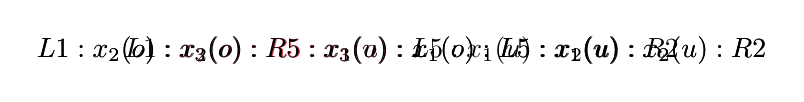
\begin{tikzpicture}
    \node<+> at(0,0){$L1:x_2(o):{\color{red}R5}:x_1(o):L5:x_1(u):x_2(u):R2$};
    \node<+> at(0,0){$L1:x_2(o):{\color{red}x_3(o):R5:x_3(u)}:x_1(o):L5:x_1(u):x_2(u):R2$};
    \node<+> at(0,0){$L1:x_2(o):{x_3(o):R5:x_3(u)}:x_1(o):L5:x_1(u):x_2(u):R2$};
\end{tikzpicture}$$
\end{frame}

\note[itemize]{
\item (2) under because our finger is going above
}

\begin{frame}{\name}
$$\scriptstyle
L1:L5:R2\enspace\xmapsto{\overset\Longleftarrow{R5}(\overline{Lp})}\enspace L1:x_2(o):{x_3(o):R5:x_3(u)}:x_1(o):L5:x_1(u):x_2(u):R2
$$

\begin{center}
\g[0.4]{figures/star-before}$\xmapsto{\overset\Longleftarrow{R5}(\overline{Lp})}$
\g[0.4]{figures/star-pick-twist}
\end{center}
\end{frame}

\section{Extension Cancellation}

\begin{frame}{\secname}
\g[0.5]{figures/ext1}
\g[0.5]{figures/ext2}
\end{frame}

% \begin{frame}{To Do}
% \begin{itemize}
%     \item Transfer your magic paragraph from the article to here
%     \item Plan out your slides to ideas / content
% \end{itemize}
% \end{frame}

\end{document}
